%=========================================================================
% (c) Michal Bidlo, Bohuslav Křena, 2008

\chapter{Úvod}
Abychom mohli napsat odborný text jasně a~srozumitelně, musíme splnit několik základních předpokladů:
\begin{itemize}
\item Musíme mít co říci,
\item musíme vědět, komu to chceme říci,
\item musíme si dokonale promyslet obsah,
\item musíme psát strukturovaně. 
\end{itemize}

Tyto a další pokyny jsou dostupné též na školních internetových stránkách \cite{fitWeb}.

Přehled základů typografie a tvorby dokumentů s využitím systému \LaTeX je 
uveden v~\cite{Rybicka}.

\section{Musíme mít co říci}
Dalším důležitým předpokladem dobrého psaní je {\it psát pro někoho}. Píšeme-li si poznámky sami pro sebe, píšeme je jinak než výzkumnou zprávu, článek, diplomovou práci, knihu nebo dopis. Podle předpokládaného čtenáře se rozhodneme pro způsob psaní, rozsah informace a~míru detailů.

\section{Musíme vědět, komu to chceme říci}
Dalším důležitým předpokladem dobrého psaní je psát pro někoho. Píšeme-li si poznámky sami pro sebe, píšeme je jinak než výzkumnou zprávu, článek, diplomovou práci, knihu nebo dopis. Podle předpokládaného čtenáře se rozhodneme pro způsob psaní, rozsah informace a~míru detailů.

\section{Musíme si dokonale promyslet obsah}
Musíme si dokonale promyslet a~sestavit obsah sdělení a~vytvořit pořadí, v~jakém chceme čtenáři své myšlenky prezentovat. 
Jakmile víme, co chceme říci a~komu, musíme si rozvrhnout látku. Ideální je takové rozvržení, které tvoří logicky přesný a~psychologicky stravitelný celek, ve kterém je pro všechno místo a~jehož jednotlivé části do sebe přesně zapadají. Jsou jasné všechny souvislosti a~je zřejmé, co kam patří.

Abychom tohoto cíle dosáhli, musíme pečlivě organizovat látku. Rozhodneme, co budou hlavní kapitoly, co podkapitoly a~jaké jsou mezi nimi vztahy. Diagramem takové organizace je graf, který je velmi podobný stromu, ale ne řetězci. Při organizaci látky je stejně důležitá otázka, co do osnovy zahrnout, jako otázka, co z~ní vypustit. Příliš mnoho podrobností může čtenáře právě tak odradit jako žádné detaily.

Výsledkem této etapy je osnova textu, kterou tvoří sled hlavních myšlenek a~mezi ně zařazené detaily.

\section{Musíme psát strukturovaně} 
Musíme začít psát strukturovaně a~současně pracujeme na co nejsrozumitelnější formě, včetně dobrého slohu a~dokonalého značení. 
Máme-li tedy myšlenku, představu o~budoucím čtenáři, cíl a~osnovu textu, můžeme začít psát. Při psaní prvního konceptu se snažíme zaznamenat všechny své myšlenky a~názory vztahující se k~jednotlivým kapitolám a~podkapitolám. Každou myšlenku musíme vysvětlit, popsat a~prokázat. Hlavní myšlenku má vždy vyjadřovat hlavní věta a~nikoliv věta vedlejší.

I k~procesu psaní textu přistupujeme strukturovaně. Současně s~tím, jak si ujasňujeme strukturu písemné práce, vytváříme kostru textu, kterou postupně doplňujeme. Využíváme ty prostředky DTP programu, které podporují strukturovanou stavbu textu (předdefinované typy pro nadpisy a~bloky textu). 


\chapter{Proteíny}

Proteíny (bielkoviny) môžeme charakterizovať ako základné stavebné prvky všetkých živých organizmov. Nie sú však iba stavebnými prvkami bunky, zabezpečujú väčšinu bunečných funkcií. Pochopenie procesu vzniku proteínov a ich funkcie nachádza široké uplatnenie v odvetviach ako medicína, poľnohospodárstvo, priemysel a mnohé ďaľšie. 
V tejto kapitole sa budem zaoberať základným rozdelením proteínov, procesom ich vzniku z DNA a štruktúrou.

\section{Základné rozdelenie proteínov}

Proteíny sú biopolyméry tvorené z jedného alebo viacerých polypeptidových reťazcov, ktoré je možné chápať ako sekvenciu polymérov aminokyselín navzájom spojených kovalentnou peptidovou väzbou. Proteíny sa skladajú do množstva komplikovaných tvarov a~ich funkcie súvisia s~konkrétnym priestorovým usporiadaním (konformáciou), pričom sa snažia zaujať čo najlepšiu konformáciu z energetického hľadiska. Konformácia vychádza z~primárnej štruktúry, ktorú môžeme chápať ako reťazec aminokyselín v~danom poradí \cite{proteiny}. Podľa funkcie môžeme proteíny rozdeliť do niekoľkých skupín \cite{proteiny}:  
\begin{itemize}
	\item \textbf{Enzýmy:} ich funkciou je katalýza rozpadu a tvorba kovalentných väzieb. Príkladom môže byť napríklad pepsín, ktorý sa podieľa na odbúraní bielkovín pri trávení.
	\item \textbf{Štruktúrne proteíny:} tvoria základné stavebné jednotky buniek a tkanív, poskytujú im mechanickú oporu. Príkladom je keratín tvoriaci základnú zložku vlasov a nechtov.
	\item \textbf{Transportné proteíny:} prenášajú malé molekuly a ionty v organizme. Príkladom sú proteín hemoglobín ako nosič kyslíka v krvnom obehu a proteín transferrin prenášajúci železo.
	\item \textbf{Pohybové proteíny:} sú pôvodcami pohybu buniek a tkanív. Príkladom takýchto proteínov sú kinesin a myosin.
	\item \textbf{Zásobné proteíny:} slúžia na skladovanie malých molekúl a iontov. Kasein v mlieku poskytuje zdroj aminokyselín pre novonarodené živočíchy. 
	\item \textbf{Signálne proteíny:} ich funkcoiu je prenos informačných signálov medzi bunkami. Do tejto skupiny patrí známy proteín inzulín regulujúci hladinu cukru v krvi.
	\item a ďaľšie.
\end{itemize}

\section{Aminokyseliny}
Aminokyseliny sú odvodené od organických kyselín a predstavujú rôzne triedy molekúl s~jednou spoločnou vlastnosťou, všetky vlastnia karboxylovú (COOH) a aminovú ($NH_{2}$) skupinu. Tieto skupiny sú naviazané k jednému uhlíkovému atómu, ktorý je označovaný ako $\alpha$ uhlík. Rôznorodosť jednotlivých aminokyselín spočíva v~postrannom reťazci (R) určujúcom chemické vlastnosti aminokyselín, resp. proteínov. Jednotlivé aminokyseliny sú v~proteínovej molekule vzájomne spojené peptidovou väzbou, ktorá prepojuje karboxylovú skupinu jednej aminokyseliny s~amino skupinou druhej. Reťazec viacerých aminokyselín je označovaný ako peptidový reťazec (polypeptid). 
Celkovo existuje 20 rôznych aminokyselín, ktoré môžeme na základe chemických vlastností postranných reťazcov rozdeliť na šesť základných skupín \cite{aminokyseliny}:

\begin{itemize}
	\item \textbf{Aminokyseliny s alifatickým postranným reťazcom:} alanin (Ala), valin (Val), leucin (Leu), isoleucin (Ile), glycin (Gly)
	\item \textbf{Bazické skupiny s aminovou skupinou na postrannom reťazci:} arginin (Arg), lysin (Lys)
	\item \textbf{S aromatickým jadrom alebo hydroxylovou skupinou na postrannom reťazci:}
	histidin (His), fenylalanin (Phe), serin (Ser), threonin (Thr), tyrosin (Tyr), tryptofan (Trp)
	\item \textbf{Kyslé skupiny s karboxylovou alebo aminovou skupinou na postrannom reťazci:} kyselina asparagová (Asp), asparagin (Asn), kyselina glutamová (Glu), glutamin (Gln)
	\item \textbf{So sírou v postrannom reťazci:} methionin (Met), cystein (Cys)
	\item \textbf{Obsahujúce sekundárny amin:} prolin (Pro)
\end{itemize}

\section{Syntéza proteínov}

Proteíny vznikajú z DNA v procese nazývanom proteosyntéza. Tento proces sa skladá z 2 hlavných častí, ktorými sú transkripcia a translácia.

\begin{itemize}

\item \textbf{Transkripcia:} pri procese transkripcie dochádza k prepisu časti nukleotidovaj sekvencie DNA (génu) do molekuly RNA. Dôležitú úlohu zohráva enzým RNA-polymeráza, ktorá musí pred začiatkom traskripcie nájsť oblasť tzv. promotoru obsahujúcu informáciu o začiatku transkripcie a následne sa na túto oblasť naviazať. Proces prepisu končí keď RNA-polymeráza narazí na sekvenciu tzv. terminátoru. Výsledná molekula RNA sa označuje ako mediátorová RNA (mRNA). 
\item \textbf{Translácia:} pri procese translácie dochádza k prenosu informácie z mRNA do polypeptidového reťazca aminokyselín. Sekvencia nukleotidov RNA sa postupne číta po trojiciach (tzv. kodónoch), pričom každý kodón je preložený na jednu z dvadsiatich aminokyselín. Trojica nukleotidov umožňuje vytvoriť 64 možných kombinácií, takže jedna aminokyselina môže byť reprezentovaná viacerými kodónmi. Výsledkom translácie je proteín.

\end{itemize}
\newpage
\section{Štruktúra proteínov}
Popis trojrozmernej štruktúry proteínov môžeme podľa \cite{aminokyseliny} rozdeliť do štyroch úrovní organizácie:

\begin{itemize}
	\item \textbf{Primárna štruktúra:} sekvencia aminokyselín v polypeptidovom reťazci
	\item \textbf{Sekundárna štruktúra:} zachytáva elementy, ktoré na krátkych úsekoch v~sekvencií proteínu zaujímajú podobnú konformáciu. Ide najmä o $\alpha$\--špirálu ($\alpha$\--helix) a $\beta$\--~štruktúra alebo ($\beta$\--skladaný list). $\alpha$\--špirála je také priestorové usporiadanie, kedy reťazec vytvára špirálu. Táto konformácia je stabilizovaná vodíkovými mostíkmi medzi peptidovými väzbami ležiacimi nad sebou \cite{bibid}. V prípade $\beta$\--štruktúry prebiehajú úseky reťazca paralelne vedľa seba a~sú stabilizované vodíkovými mostíkmi medzi susediacimi úsekmi.
	\item \textbf{Terciálna štruktúra:} reprezentuje trojrozmerné priestorové usporiadanie zloženého polypeptidového reťazca \cite{aminokyseliny}. Na podobe výslednej terciálnej štruktúry majú vplyv chemické vlastnosti aminokyselín a ich usporiadanie v reťazci. 
	\item \textbf{Kvartérna štruktúra:} popisuje usporiadanie jednotlivých polypeptidových reťazcov v molekule proteínu. Týka sa to však iba tzv. oligomerných proteínov, ktoré sú tvorené z viac ako jedného polypetidového reťazca.
	
	Primárnu, sekundárnu, terciálnu a kvartérnu štruktúru je možné vidieť na obrázku \ref{struktura}:
\end{itemize}
\begin{figure}[H]
		\begin{center}
		\scalebox{0.5}
		{   
			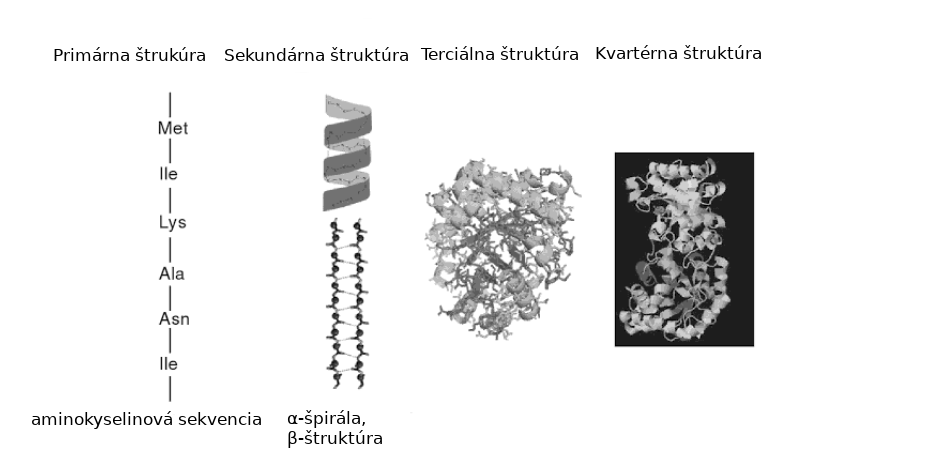
\includegraphics{structure.png}
		}
		\caption{Primárna, sekundárna, terciálna a kvartérna štruktúra. Prevzaté a upravené z \cite{gromiha}.}
		\label{struktura}
	\end{center}
\end{figure}

\chapter{Vplyv aminokyselinových substitúcií na stabilitu proteínu}

Stabilita je jednou z najdôležitejších vlastností proteínu. Motivácia skúmania stability je dnes veľká, pretože táto vlastnosť proteínov je dôležitá v mnohých oblastich ako je medicína, kde chceme dosiahnuť výrobu účinnejších liečiv, v oblasti priemyslu a poľnohospodárstva. Stabilný proteín dokáže lepšie znášať nepriaznivé podmienky okolitého prostredia, akými sú vyššie teploty alebo chemické vlastnosti okolia v ktorom sa proteín nachádza. Na stabilitu proteínu však vplývajú aminokyselinové substitúcie, ktoré môžu proteín stabilizovať, ale aj destabilizovať. Preto vzniká potreba skúmať vplyv substitúcií na stabilitu. V tejto kapitole sa zmienim o stabilite proteínu, čo stabilitu určuje a o dôvodoch vzniku a vplyve mutácií.


\section{Stabilita proteínu}
Stabilita proteínu je určená množinou vzájomne pôsobiacich a ovplyvňujúcich sa síl. Tieto sily určujú, či sa proteín nachádza vo svojom pôvodnom zloženom alebo rozloženom (denaturovanom) stave. Stabilita je úzko prepojená so stavom, v ktorom sa proteín nachádza. Stabilný proteín sa nachádza v zloženom stave, ktorý je stabilizovaný rôznymi vzájomnými interakciami, kde patria hydrofóbne, elektrostatické, vodíkové väzby alebo van der Waalsove sily. Naopak, nestabilný proteín sa nachádza v denaturovanom stave, kde dominuje entropická a neentropická voľná energia. \cite{gromiha}

Stabilitu proteínu je možné reprezentovať ako zmenu tzv. Gibbsovej (voľnej) energie ($\Delta$G) potrebnej na prechod proteínu zo zloženého do denaturovaného stavu alebo naopak. 
Gibbsova voľná energia je termodynamický potenciál vyjadrujúci maximálne množstvo reverzibilnej práce, ktorá môže byť uskutočnená termodynamickým systémom pri konštantnej teplote a tlaku. Gibbsova voľná energia je definovaná nasledujúcim vzťahom \cite{gibbs}:
\begin{align}
	G = H - TS,
\end{align}
kde $H$ predstavuje entalpiu, $T$ teplotu a $S$ entropiu.

Zmena voľnej Gibbsovej energie ($\Delta G$) je dana vzťahom
\begin{align}
	\Delta G = G_{folded} - G_{unfoldeded},
\end{align}
kde $G_{folded}$ predstavuje voľnú energiu v zloženom a $G_{unfolded}$ energiu v nezloženom stave.
  Existuje niekoľko laboratórnych metód na určenie stability ako napríklad cirkulárny dichroizmus (CD), diferencilna skenovacia kalorimetria (DSC), fluorescencia (Fl), absorpcia svetla (Abs), nukleárna magnetická rezonancia (NMR) \cite{gromiha}.

Určenie stability bez použitia niektorej z laboratórnych metód je možné uskutočniť výpočtom jedného z existujúcich silových polí (Talaris, Score12, ...). Výpočet takéhoto poľa ukazuje nasledujúci jednoduchý príklad \cite{free_energy} \cite{gromiha}:

Voľná energia v zloženom stave je daná vzťahom  
	\begin{align}
		G_{F} = G_{hy} + G_{el} + G_{hb} + G_{vw} + G_{ss},
	\end{align}

kde $G_{hy}, G_{el}, G_{hb}, G_{ss}, G_{vw}$ sú hydrofóbne, elektrostatické, vodíkové, disulfidické a van der Waalsove voľné energie. 


Elektrostatickými interakciami najviac prispievajú nabité postranné reťazce reziduí Lysine, Hystodine, Arginine a kyselina asparagová a glutamová.

Vodíkové väzby sú jednými z hlavných zúčastnených pri tvorbe sekundárnej štruktúry proteínu. Výpočet ich príspevku je založený najmä na ich geometrických informáciách.

Voľná energia v nezloženom stave je daná vzťahom
\begin{align}
	G_U = G_{en} + G_{ne},
\end{align}
kde $G_{en}$ a $G_{ne}$ sú entropické a neentropické voľné energie.


\section{Mutácie}
Mutácie sú náhodné alebo cielené zmeny v DNA. Sú naprosto nevyhnutné pre biologickú evolúciu, bez nich by sa skôr či neskôr zastavila. Ak by sa výraznejšie zmenili podmienky vonkajšieho prostredia, organizmy by bez mutácií nemuseli na zmeny zareagovať a pravdepodobne by vyhynuli. Mutáciami sú označované všetky také zmeny genetickej informácie, ktoré nie sú výsledkom segregácií a rekombinácií už existujúcich častí genotypov \cite{mutace}. 
Podľa úrovne, na ktorej sa mutácia vyskytla, môžeme rozlišovať \cite{flegr}:
\begin{itemize}
	\item \textbf{Génové mutácie:} zmena v stavbe DNA, ktorá je reprezentovaná zmenou nukleotidovej sekvencie na určitom mieste \cite{mutace}. Nazývajú sa tiež bodovými mutáciami a z hľadiska predikcie sú najzásadnejšie.
	\item \textbf{Chromozómové mutácie:} mení sa štruktúra chromozómu.
	\item \textbf{Genónové mutácie:}  mení sa počet chromozómov.
\end{itemize}

\subsection{Vznik mutácií}

Mutácie nevznikajú náhodne, každá mutácia má svoju príčinu za ktoru stojí pôsobenie tzv. mutagénnych faktorov. Medzi najdôležitejšie patria chemické a fyzikálne faktory.

Medzi fyzikálne faktory patria rôzne zdroje žiarenia, najmä ionizujúce a ultrafialové. Poškodenie štruktúry DNA je priamo úmerné množstvu absorbovaného žiarenia.

Medzi chemické faktory môžeme zaradiť genotoxické látky, tzv. genotoxíny. Takýchto látok je veľké množstvo a patria medzi ne napríklad pesticídy, herbicídy, niektoré farbivá, konzervačné a dezinfekčné látky \cite{mutace}. 

\subsection{Typy mutácií}

Podľa \cite{flegr} rozlišujeme tri základné typy génových mutácií:
\begin{itemize}
	\item \textbf{Substitúcia:} jedná sa o zámenu jedného alebo viacerých párov po sebe nasledujúcich bází inými \cite{mutace}. V tomto prípade sa nemení dĺžka pôvodného proteínu. Novovziknutý proteín sa obvykle líši v jednej aminokyseline oproti pôvodnému. 
	\item \textbf{Vloženie:} jedná sa o vloženie jedného alebo viacerých nových párov bází do pôvodnej sekvencie, spôsobuje zväčšenie dĺžky sekvencie.
	\item \textbf{Odstránenie:} odstránenie jedného alebo viacerých po sebe nasledujúcich párov bází, mení dĺžku sekvencie rovnako ako inzercia.
\end{itemize}

\begin{figure}[H]
	\centering
	\begin{center}
		\scalebox{0.6}
		{   
			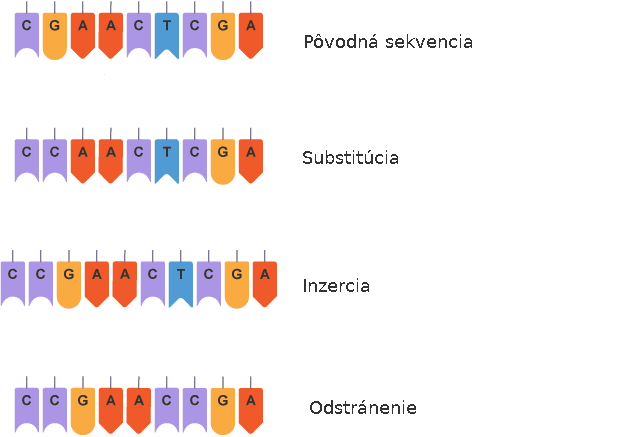
\includegraphics{mutation_types.png}
			%https://www.bbc.co.uk/education/guides/zc499j6/revision/2
		}
		\caption[mutacie]{Jednotlivé typy mutácií\footnotemark.}
	\end{center}
\end{figure}
\footnotetext{Zdroj: \url{https://www.bbc.co.uk/education/guides/zc499j6/revision/2}}

V prípade, že k mutácií dôjde v kódujúcej oblasti, môžeme mutácie rozlíšiť na \cite{flegr}:
\begin{itemize}
	\item \textbf{Synonymné:} vychádzajú z tzv. degenerovanosti genetického kódu. Zámena nukleotidu v kodóne sa tak na štruktúre proteínu nemusí vôbec prejaviť a vyzerá to tak, ako keby k mutácií vôbec nedošlo. 
	\item \textbf{Nesynonymné:} pri zmene nukleotidu v kodóne dochádza k zmene aminokyseliny a rovnako aj k zmene konformácie proteínu.
	\item \textbf{Posunové:} spôsobujú zmenu čítacieho rámca a často vedú k predčasnému ukončeniu prekladu proteínu.
	\item \textbf{Nezmyselné:} vytvárajú STOP kodón a tým spôsobujú predčasné ukončenie prekladu proteínu.
\end{itemize}
\newpage
Na stabilitu proteínu vplývajú aminokyselinové mútacie, ktoré môžu spôsobiť to, že proteín sa stane nestabilným. Preto do hlavnej oblasti skúmania stability patrí predikcia zmeny stability na základe aminokyselinovej mutácie. Jedná sa o predikciu zmeny Gibbsovej voľnej energie ($\Delta\Delta$G) medzi voľnou energiou pôvodného a zmutovaného proteínu. Môžeme ju definovať nasledujúcim vzťahom:
\begin{align}
	\Delta\Delta G = G_{mutant} - G_{wild\_type},
\end{align}
Podľa tejto hodnoty je možné rozdeliť mutácie na stabilizujúce, neutrálne a destabilizujúce. Väčšia snaha pri predikcií môže viesť k zlepšeniu návrhu nových odolnejších proteínov alebo pri štúdií rozličných chorôb.



\chapter{Strojové učenie}
\label{ml}
Strojové učenie je v súčasnej dobe chápané ako disciplína umelej inteligencie. Základnou technikou strojového učenia je prehľadávanie stavového priestoru. K charakteristickým vlastnostiam patrí využívanie znalostí, práca so symbolickými či štruktúrovanými premennými \cite{machine_learning}. Pojem strojové učenie takisto označuje počítačové metódy pracujúce s obrovským množstvom dát, medzi ktorými je snahou nájsť vzťahy. Takéto metódy nachádzajú svoje uplatnenie pri hľadaní riešení v mnohých odvetviach akými sú počítačové videnie, rozpoznávanie reči a takisto bioinformatika. Keďže strojové učenie nachádza v mnohých odvetviach čoraz väčšie uplatnenie, je potrebné brať do úvahy jeho výhody a rovnako aj nevýhody. Medzi výhody patrí automatické hľadanie vzťahov vo veľkom množstve dát, čo by bolo pri mechanickom hľadaní takmer nemožné. Medzi hlavné nevýhody metód patrí neschopnosť správnej analýzy dát pri nevyváženosti predložených dát, nesprávne výsledky pri malom množstve tréningových dát pre metódu alebo nemožnosť práce s dátami obsahujúcimi veľké množstvo parametrov.

V tejto kapitole sa budem venovať základným technikám strojového učenia a popisom používaných algoritmov. 

\section{Úvod do strojového učenia}

Podľa \cite{alpaydin} je možné algoritmy strojového učenia rozdeliť do 3 základných skupín:
\begin{itemize}
	\item \textbf{Klasifikácia:} Rieši problém priradenia výstupnej triedy vstupným dátam, ktoré môžu byť reprezentované vektorom hodnôt. Ako príklad si je možné predstaviť zatriedenie žiadateľov o pôžičku do tried s vysokým alebo nízkym rizikom toho, že pôžičku nebudú schopní splácať na základe rôznych údajov o žiadateľoch.
	\item \textbf{Regresia:} Regresné metódy narozdiel od klasifikačných nepriraďujú vstupom výstupnú triedu, ale snažia sa určiť priamo číselnú hodnotu výstupu. Príkladom môže byť určenie ceny ojazdeného auta na základe parametrov ako počet najazdených kilometrov, značka, rok výroby.
	\item \textbf{Hľadanie asociácií:} Asociačné pravidlá slúžia na hľadanie zaujímavých asociácií vo veľkom objeme dát. Pri ich hľadaní nás zaujíma podmienená pravdepodobnosť, ktorá sa uvádza vo forme $P(X|Y)$, $Y$ je produkt podmienený výskytom produktu $X$. 
\end{itemize}


Metódy strojového učenie môžeme ďalej rozdeliť na základe spôsobu, akým sa učia. Podľa \cite{alpaydin} ich rozdeľujeme na:
\begin{itemize}
	\item \textbf{Učenie s učiteľom:} Pri tomto type učenia je nutné mať k dispozícií vstupné aj výstupné dáta. Cieľom je nájsť vzťahy medzi vstupom a výstupom, ktoré slúžia na naučenie metódy. Medzi algoritmy patriace do tejto skupiny radíme regresiu aj klasifikáciu.
	\item \textbf{Učenie bez učiteľa:} V tomto type učenie nie sú k dispozícií referenčné výstupné dáta, ale len vstupné. Snahou je nachádzať pravidelnosti vo vstupných dátach. Medzi takéto metódy patria rôzne typy zhlukovania. 
\end{itemize}

\section {Rozhodovacie stromy}
Rozhodovací strom je hierarchický model so stromovou štruktúrou. Metódy tohto typu používajú učenie s učiteľom a môžeme ich použiť na klasifikáciu aj regresiu. Štruktúra stromu je tvorená z dvoch typov uzlov, vnútorných (nelistových) a listových uzlov. Každý z nelistových uzlov obsahuje testovaciu funkciu. Po vyhodnotení tejto funkcie sa vyberie nasledujúci uzol, v ktorom sa bude pokračovať. Tento proces začína v koreňovom uzle a pokračuje rekurzívne až do dosiahnutia listového uzlu. Listový uzol obsahuje označenie triedy do ktorej bude zaradený vstupný vektor alebo číselnú hodnotu.

\subsection{Algoritmus J48}

Algoritmus J48 patrí k metódam rozhodovacích stromov. Algoritmus produkuje klasifikačno-~rozhodovací strom pre poskytnuté dáta rekurzívnym rozdeľovaním dát. Pri rozhodovaní je využitá stratégia depth-first. Algortimus berie do úvahy všetky možné testy, ktoré môžu rozdeliť dáta a vyberá test udávajúci najlepšiu informačnú hodnotu. Pre každý diskrétny atribút je zvážený jeden test s počtom výsledkov, ktorý zodpovedá počtu rôznych hodnôt atribútov. 
%výsledkami pre taký počet hodnôt, koľko je rôznych hodnôt atribútov. 

\subsection{Algoritmus Náhodný strom (Random Tree)}

Pri tomto algoritme je strom náhodným stromom vytvoreným náhodne z množstva všetkých možných stromov. Každý list obsahuje $k$ náhodných parametrov. Náhodné vytvorenie stromu v tomto kontexte znamená, že každý strom v množine stromov má rovankú šancu výberu. Kombinácia veľkého počtu náhodných stromov obvykle vedie k správnemu modelu. 

\subsection{Algoritmus Náhodný les (Random Forest)}

Random Forest \cite{breiman} je metóda založená na kombinácií viacerých rozhodovacích stromov. Každý strom závisí na hodnotách náhodného vektora hodnôt navzorkovaného nezávisle a s rovnakým rozložením pre všetky stromy v tzv. lese stromov. Obecne môžeme metódu popísať nasledujúcou definíciou:

Náhodný les (random forest) je klasifikátor tvorený kolekciou klasifikátorov so stromovou štruktúrou $\{h(x,\Theta_{k}), k=1, ...\}, $ kde $\{k\}$ sú nezávisle identicky rozdelené náhodné vektory a každý strom hlasuje jednotlivo o najpopulárnejšej triede vo vstupe $x$.
\newpage
Najväčšiu pozornosť tejto metódy tvoria 3 vlastnosti:
\begin{itemize}
	\item poskytuje presnú predikciu pre mnohé typy aplikácií
	\item je schopná merať dôležitosť jednotlivých parametrov pri trénovaní modelu
	\item blízkosť medzi vzorkami môže byť meraná trénovaným modelom
\end{itemize} 

Algoritmus náhodný les pre klasifikáciu aj regresiu môžeme zjednodušene popísať nasledovne, pričom uvažujeme $M$ rozhodovacích stromov. Schéma metódy je znázornená na obrázku \ref{random_forest}:
\begin{itemize}
	\item Pre každý z $M$ rozhodovacích stromov vytvoríme sadu tréningových dát z originálnych dát. Na ich výber slúži metóda tzv. bagging, ktorá náhodne vyberie zadaný počet trénovacích dát.
	\item Pre každú množinu tréningových dát vytvoríme klasifikačný alebo regresný strom, ktorý je následne natrénovaný na $M$-tej náhodnej množine tréningových dát. V tejto metóde je každý uzol rozdelený najlepším rozdelením spomedzi podmnožiny prediktorov náhodne vybraných v tomto uzle. Naopak, pri klasických stromoch je uzol rozdelený na základe najlepšieho rozdelenia medzi všetkými premennými.
	\item Predikcia nových dát spojením výsledkov predikcie M stromov, napríklad hlasovaním väčšiny (tzv. majority voting) pri klasifikácií alebo priemerom hodnôt pri regresí.
\end{itemize}

Rozšírenie algoritmu náhodný les je momentálne veľmi aktívnou oblasťou vo výpočetnej biológií. Metóda nachádza veľké uplatnenie v bioinformatike, napríklad aj pri nástrojoch predikujúcich stabilitu proteínov.

\begin{figure}[H]
	\centering
	\begin{center}
		\scalebox{0.8}
		{   
			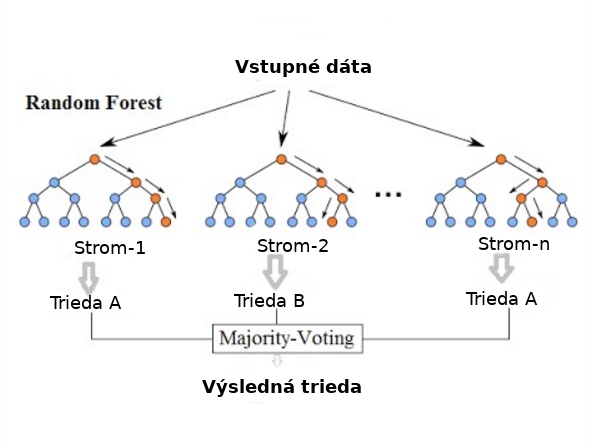
\includegraphics{rf.png}
			%https://d2wh20haedxe3f.cloudfront.net/sites/default/files/random_forest_diagram_complete.png
		}
		\caption[Random Forest]{Metóda Random Forest\footnotemark.}
		\label{random_forest}
	\end{center}
\end{figure}
\footnotetext{Zdroj: \url{http://bit.ly/2rpjSDK}}

\section {Support vector machines (SVM)}

Support vector machines patria k najnovším metódam strojového učenia. Tieto metódy uskutočňujú klasifikáciu konštruovaním N-dimenzionálnej nadroviny, ktorá optimálne rozdeľuje dáta do dvoch kategórií. Cieľom je nájsť takú nadrovinu, ktorá rozdelí vstupné vektory tak, že jedna skupina vektorov je na jednej strane roviny a druhá na strane opačnej. Vektory nachádzajúce sa blízko nadroviny označujeme ako tzv. podporné vektory (support vectors). 

Ak sú trénovacie dáta lineárne rozdeliteľné, potom pár $(\textbf{w},b)$ existuje ako 

	$\textbf{w}^{T}\textbf{x}_{i} + b \geq 1$, pre všetky $\textbf{x}_{i} \in P$
	
    $\textbf{w}^{T}\textbf{x}_{i} + b \leq -1$, pre všetky $\textbf{x}_{i} \in N$
    
s rozhodovacím pravidlom daným vzťahom $f_{\textbf{w},b} ( x ) = sgn(\textbf{w}^{T}x + b )$, kde $\textbf{w}$ je váhový vektor a $b$ je odchýlka (tzv. bias).

V prípade, že dáta sú lineárne rozdeliteľné do dvoch tried, optimálnu nadrovinu je možné nájsť minimalizovaním štvorcovej normy rozdeľujúcej nadroviny. Jedná sa o konvexný kvadratický programovací problém.
Pri možnosti lineárneho rozdelenia sa snaží SVM nájsť 1-dimenzionálnu nadrovinu (priamku), ktorou rozdelí skupiny vstupných vektorov. Po rozdelení dát priamkou metóda zistí vzdialenosť priamky od najbližších podporných vektorov. Táto vzdialenosť sa označuje ako tzv. krajná hranica (margin), pričom sa hľadá najväčšia vzdialenosť medzi podpornými vektormi.  

Lineárne rozdeliteľné dáta sú však len ideálnym príkladom. Ak by analýza pozostávala len z premenných z dvoch kategórií, dvoch predikovaných premenných a množiny bodov rozdeliteľných priamkou, bolo by to veľmi jednoduché. V skutočnosti sa tieto metódy musia vysporiadať s viac ako dvomi predikovanými premennými, rozdelením dát nelineárnymi krivkami alebo množinami dát, ktoré nemôžeme úplne rozdeliť. 

\subsection{Jadrové funkcie}

Pri väčšine reálnych problémov neexistuje lineárna nadrovina rozdeľujúca pozitívne a negatívne vzorky v tréningových dátach. Jedným z riešení je prenesenie dát do priestoru, ktorý má viac dimenzí a definovať rozdeľujúcu nadrovinu v tomto priestore. Takýto viacdimenzionálny priestor sa nazýva priestor transformovaných vlastností. S vhodne vybraným priestorom transformovaných vlastností dostatočnej dimenzie je možné rozdeliť ľubovoľnú tréningovú dátovú sadu.
Mapovanie dát do iného (potencionálne nekonečného) Hilbertovho priestoru H je definované ako $\Phi:R^{d} \rightarrow H$. Trénovací algoritmus bude potom závisieť len na dátach skrz bodové produkty v H, napríklad na funkciách v tvare $\Phi(x_{i})\cdot\Phi(x_{j})$. Ak by existovala tzv. jadrová funkcia K taká, že $K(x_{i},x_{j}) = \Phi(x_{i})\cdot\Phi(x_{j})$, v algoritme by sme potrebovali iba K. 

Jadrové funkcie sú špeciálnou triedou funkcií umožňujúce výpočet vnútorných produktov priamo v priestore vlastností bez nutnosti mapovania dát tak ako to bolo popísané vyššie. 
Akonáhle je vytvorená nadrovina, jadrová funkcia je použitá na mapovanie nových bodov do priestoru vlastností pre klasifikáciu.
\newpage
Výber vhodnej aproximačnej jadrovej funkcie je dôležitý, pretože funkcia definuje transformovaný priestor vlastností v ktorom budú klasifikované tréningové dáta. Medzi najpoužívanejšie jadrové funkcie patria
\begin{itemize}
	\item $K(x,y) = (x \cdot y + 1)^{P}$
	\item $K(x,y) = e^{- {\parallel x - y \parallel}^{2}/ {2\sigma}^{2}}$
	\item $K(x,y) = tanh (\kappa x \cdot y -\delta)^{P}$
\end{itemize}


\subsection{Algoritmus SMO}

Sekvenčná minimalizačná optimalizácia (SMO) je algoritmus na trénovanie SVM, ktorý jednoducho rieši kvadratický SVM problém. SMO uskutočňuje dekompozíciu celkového problému na podproblémy riešené analyticky. Metóda si v každom kroku vyberá na vyriešenie najmenší optimalizačný problém. Pre typický kvadratický SVM problém, najmenší možný optimalizačný problém zahŕňa dva Lagraengove násobitele. V každom kroku si metóda vyberia dva tieto násobitele na spoločnú optimalizáciu, nájde pre ne optimálne hodnoty a aktualizuje SVM. Výhodou tohto algoritmu je, že množstvo potrebnej pamäte pri trénovacej sade je lineárne, čo umožňuje algoritmu pracovať s veľkými tréningovými sadami. 
 
\section{Algoritmus Naive Bayes}

Naive Bayes je klasifikačným algoritmom pre klasifikačné problémy, kde sa vyskytujú dve alebo viac tried. Je založený na Bayesovom teoréme s nezávislými predpokladmi medzi prediktormi. Klasifikátor predpokladá, že efekt hodnoty $x$ prediktoru na danú triedu $c$ je nezávislý na hodnotách ďaľších prediktorov. Predpoklad sa nazýva triedna podmienená nezávislosť. 

Tento model je jednoduchý na vytvorenie, no napriek svojej jednoduchosti klasifikátor často poskytuje dobré výsledky a je široko používaný, pretože v mnohých prípadoch prekonáva komplikovanejšie klasifikačné metódy.

\chapter{Ensemble metódy}

V posledných rokoch sa metódy strojového učenia využívajú vo veľkej miere v oblasti bioinformatiky. Napriek ich výhodám narážame na rôzne problémy spojené najmä s nedostatkom dát, veľkou rôznorodosťou dát alebo tzv. preučením metód. Jedným z riešení, ktoré vykazujú dobré výsledky, je využitie výstupov z viacerých klasifikátorov namiesto použitia jedného samostatného klasifikátora. Takáto kombinácia môže niekedy poskytnúť protichodné výsledky a tým pomôže zvýšiť presnosť a robustnosť predikcie. Prístup využitia viacerých klasifikátorov označujeme ako tzv. ensemble.

Podľa \cite{polikar} existuje mnoho teoretických a praktických dôvodov na použitie ensemble systémov:
\begin{itemize}
	\item \textbf{Štatistické dôvody:} Dobrý výkon metódy na trénovacích dátach nemusí predpovedať dobrú výkonnosť zovšeobecňovania. Množina klasifikátorov s podobným výkonom na trénovacích dátach môže mať rôznu zovšeobecňovaciu výkonnosť. Tento poznatok je možné vidieť najmä ak testovacie dáta určené na rozlíšenie schopnosti zovšeobecňovať nie sú dostatočne reprezentatívne. V takýchto prípadoch môže spriemerovanie výstupov niekoľkých klasifikátorov znížiť riziko zlého výberu alebo slabého klasifikátoru. 
	\item \textbf{Veľký objem dát:} V určitých oblastiach môže nastať problém príliš veľkého objemu dát, ktorý má byť spracovaný. To nie je niekedy možné efektívne uskutočniť len pomocou jedného klasifikátora. V takýchto situáciách je vhodné zvážiť rozdelenie dát na menšie celky, trénovať klasifikátory na menších celkoch a skombinovať ich výstupy pomocou vhodného kombinačného pravidla.
	\item \textbf{Malý objem dát:} Dostupnosť dostatočného a reprezentatívneho mmnožstva tréningových dát je dôležitá pre klasifikačný algoritmus, aby bol schopný dosiahnuť úspešného naučenia rozdelenia dát. Pri nedostatku tréningových dát sa osvedčili techniky prevzorkovania, ktoré sú vhodné na vytvorenie náhodných prekrývajúcich sa podmnožín dostupných dát a každú je možné použiť na učenie iného klasifikátora.
	\item \textbf{Rozdeľuj a panuj:} Napriek dostatku dát sú niektoré problémy pre klasifikátory príliš zložité, napríklad rozhodovacia hranica rozdeľujúca dáta môže byť veľmi komplexná alebo leží mimo oblasti funkcií dostupných pre vybraný klasifikačný model. Ako príklad je možné uviesť dáta, ktoré nie je možné lineárne rozdeliť. Žiadny lineárny klasifikátor nie je schopný dáta rozdeliť, avšak vhodná kombinácia lineárnych klasifikátorov tzv. ensemble systému by bola schopná naučiť sa túto nelineárnu hranicu. Dáta sú v tomto prípade rozdelené na menšie celky, pričom každý klasifikátor sa učí jednu z častí.
\end{itemize}


\section{Tvorba ensemble systémov}

Existujú dva základné spôsoby, ako vybrať členov ensemble systému: bagging a boosting. Príklad ensemble systému je možné vidieť na obrázku \ref{ensemble}.

\subsection{Bagging}

Bagging \cite{breiman2} alebo aj tzv. bootstrap aggregation je jednou z najstarších, ľahko implementovateľných ensemble stratégií. Bola navrhnutá na zlepšenie presnosti algoritmov strojového učenia používaných pri  štatistickej klasifikácií a regresií. Rôznorodosť je dosiahnutá využitím tzv. bootstrap podmnožín tréningových dát, pričom rôzne tréningové množiny sú vybrané náhodne s náhradou z celého množstva tréningových dát. Každá takáto podmnožina je určená na trénovanie iného klasifikátora rovnakého typu. Nakoniec sa využije hlasovania väčšiny na výsledkoch jednotlivých klasifikátorov. Trieda vybraná najväčším počtom klasifikátorov sa stáva konečným rozhodnutím ensemble systému.

Bagging je výkonným mechanizmom najmä pri obmedzenom množstve spoľahlivých dát. Na zaisteneie dostatočného množstva tréningových vzorkov v podmnožinách je približne 75 až 100\% vzorkov prítomných v každej podmnožine. Nastáva tak veľký prekryv medzi tréningovými podmnožinami a mnoho vzorkov sa nachádza viackrát v danej podmnožine. V takomto prípade sa rôznorodosť zaistí použitím nestabilného klasifikačného modelu pre ktorý je možné získať rôzne rozhodovacie hranice s rôznymi tréningovými dátami. Techniky ako neurónové siete alebo rozhodovacie stromy sú dobrými príkladmi na tento účel, pretože ich nestabilnosť je kontrolovateľná výberom ich parametrov.

\subsection{Boosting}

Boosting \cite{boosting} je ďaľším algoritmom na výber členov ensemble systému. Bolo dokázané, že slabý klasifikátor (iba o niečo úspešnejší ako náhodné hádanie) je možné pretvoriť na silný klasifikátor, ktorý poskytuje správne predikcie pre všetky prípady z ľubovoľne malej časti prípadov. Rovnako ako bagging, boosting vytvára súbor klasifikátorov prevzorkovaním dát s použitím hlasovania väčšiny. Prevzorkovanie je pri boostingu zlepšené, aby každému klasifikátoru boli poskytnuté najviac informatívne trénovacie dáta. Boosting vytvára tri slabé klasifikátory:
\begin{itemize}
	\item Prvý klasifikátor $C_{1}$ je trénovaný na náhodnej podmnožine dostupných dát.
	\item Tréningová podsada pre klasifikátor $C_{2}$ je vybraná ako najinformatívnejšia podsada vo vzťahu k $C_{1}$. Klasifikátor $C_{2}$ je teda trénovaný na dátach, na ktorých mal $C_{1}$ polovičnú úspešnosť. 
	\item Tretí klasifikátor $C_{3}$ je trénovaný na dátach, kde $C_{1}$ a $C_{2}$ nesúhlasili.
	\item Nakoniec sú klasifikátory skombinované hlasovaním väčšiny.
\end{itemize}

\begin{figure}[H]
	\centering
	\begin{center}
		\scalebox{0.4}
		{   
			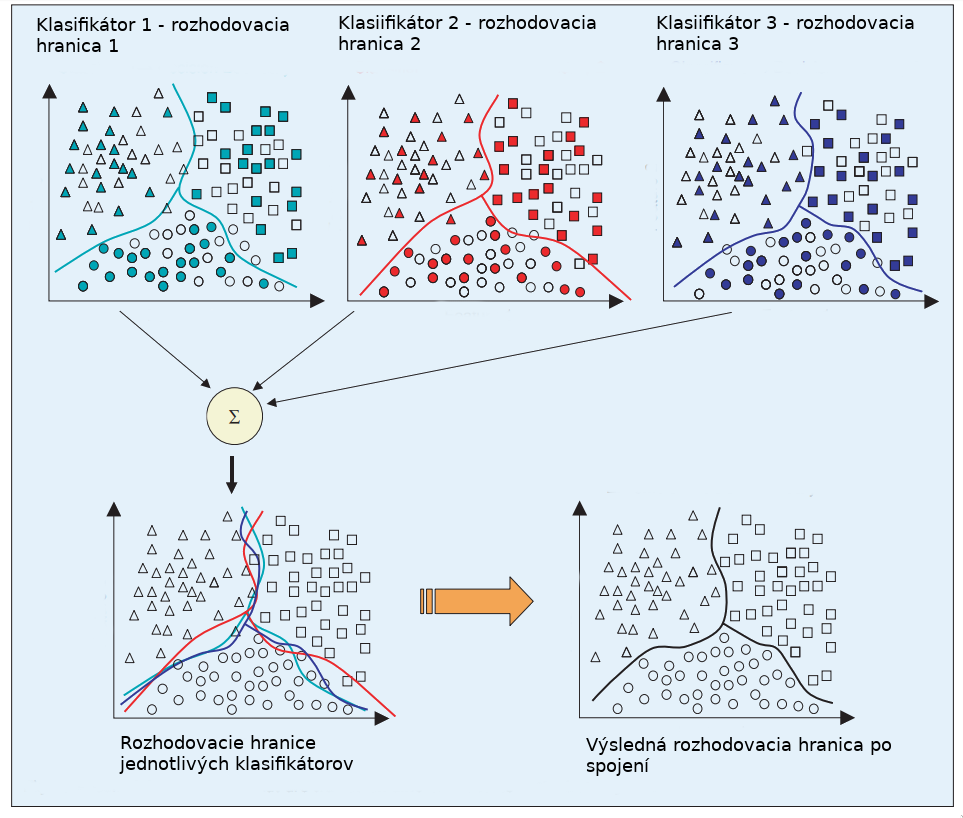
\includegraphics{ensemble.png}
			%https://www.bbc.co.uk/education/guides/zc499j6/revision/2
		}
		\caption[ensemble]{Ensemble systém. Prevzaté a upravené z \cite{polikar}.}
		\label{ensemble}	
\end{center}
\end{figure}

\section{Spojenie klasifikátorov}

Po natrénovaní jednotlivých klasifikátorov je potrebné ich spojiť najvhodnejším spôsobom. Tieto metódy môžeme rozdeliť do dvoch kategórií: netrénovateľné a trénovateľné. Netrénovateľné sú použiteľné, ak samostatný klasifikátor poskytuje porovnateľné výsledky vo väčšine častí priestoru vlastností. Trénovateľné metódy dynamicky menia rozhodovacie pravidlá podľa špecifického typu klasifikovaného prípadu, sú užitočné v prípadoch, keď klasifikátory konštantne správne alebo nesprávne klasifikujú určité prípady.

\subsection{Trénovateľné metódy}
Medzi trénovateľné metódy patria nasledovné:
\begin{itemize}
	\item \textit{Stacked generalization:} Snahou je vytvoriť metaklasifikátor s využitím poznatkov o presnoti klasifikátorov. Dostupné dáta sú rozdelené na tréningovú a testovaciu sadu. Všetky nástroje sú trénované na tréningovej sade, testovacia sada je použitá na určenie výkonnosti klasifikátorov a tvorbu metaklasifikátoru
	\item \textit{Rozhodcovské stromy:} Jedná sa o prístup zdola nahor prí tvorbe ensemble systému. V prvom kroku sú dáta rozdelené do konečného počtu neprekrývajúcich sa podsád a každá z nich je určená na trénovanie toho istého typu klasifikátora. Pre každý pár je vytvorený tzv. rozhodca a proces sa rekurzívne opakuje pokým nezostane len jeden klasifikátor na aktuálnej úrovni. 
\end{itemize}

\subsection{Netrénovateľné metódy}

Do kategórie netrénovateľných metód môžeme zaradiť nasledujúce metódy:
\begin{itemize}
	\item \textit{Hlasovanie väčšiny:} Najjednoduchšia metóda, ktorá priradí objektu triedu na základe počtu hlasov jednotlivých klasifikátorov. Existujú 3 typy: jednotné hlasovanie, kde sa všetky klasifikátory musia zhodnúť na predikcií; jednoduché hlasovanie v ktorom sa aspoň polovica klasifikátorov musí zhodnúť na rozhodnutí; väčšinové hlasovanie kde je výsledok daný podľa počtu hlasov.
	\item \textit{Váhované hlasovanie väčšiny:} Tento prístup je vylepšením predchádzajúceho prístupu, jednotlivé klasifikátory majú rôznu váhu v konečnom rozhodovaní a tieto váhy by mali byť prispôsobené ich presnosti.
	\item \textit{Bayesova kombinácia:} Váhovaná metóda, váha spojená s klasifikátorom je tzv. posterior pravdepodobnosť klasifikátora na tréningovej sade.
	\item \textit{Váhovanie entropie:} Rovnako sa jedná o váhovanú metódu a váhy klasifikátorov sú nepriamo úmerné entropií klasifikačného vektoru.
\end{itemize}


\chapter{Nástroje na predikciu stability}

Ako je už uvedené v kapitole \ref{ml}, strojové učenie nachádza čoraz väčšie uplatnenie v rôznych oblastiach akou je aj bioinformatika. V oblasti skúmania a predikcie stability vzniká mnoho nástrojov využívajúcich práve rôznych techník a metód strojového učenia. Takéto nástroje sú však zatiaľ len vo svojich začiatkoch a majú mnoho nedostatkov spojených najmä s potrebnými dátami. Ďaľšou skupinou nástrojov na predikciu stability sú také, ktoré využívajú tzv. silové polia. Túto skupinu nástrojov môžeme rozdeliť na také, ktoré využívajú fyzikálne efektívne energetické funkcie simulujúce základné sily pôsobiace medzi atómami a na metódy založené na štatistických potenciáloch, pre ktoré sú energie odvodené z výskytu reziduí alebo atómoých spojoch uvedených v dátových sadách pozostávajúcich z experimentálne charakterizovaných mutovaných proteínov.
V tejto kapitole sa zameriam na stručné zhodnotenie a opis rôznych predikčných nástrojov patriacich do vyššie uvedených kategórií.

\section{Strojové učenie}

Strojové učenie nachádza čoraz širšie uplatnenie v bioinformatike a mnohé predikčné nástroje ho využívajú ako svoj základ. V tejto sekcií sa nachádza charakteristika nástrojov využívajúch práve metódy strojového učenia.

\subsection{AUTO-MUTE}

Nástroj využíva klasifikačné metódy na určenie vplyvu mutácie a~regresiu na určenie hodnoty $\Delta\Delta G$.
Na začiatku je identifikovaných šesť najbližších susedov aminokyseliny na mutovanej pozícií a~určia sa ich vlastnosti. Vektor vlastností, tvorený vlastnosťami založenými na energií, je určený na natrénovanie vybranej metódy zvolenej užívateľom. Nástroj využíva algoritmy z~balíka programu WEKA, konktrétne je možné zvoliť metódy Random Forest a~SVM pre klasifikáciu alebo Tree Regression a~SVM Regression pre regresiu. AUTO-MUTE je dostupný ako webový server alebo ako samostatná aplikácia \cite{automute}.

\subsection{I-Mutant}

Nástroj poskytuje predikciu znamienka zmeny stability pomocou klasifikácie a~tiež určenie hodnoty $\Delta\Delta G$ pomocou regresie. I-Mutant pracuje so štrukturálnymi alebo sekvenčnými informáciami o mutovanej aminokyseline a~jej najbližších susedoch. Pre strojové učenie je použitá metóda SVM s~jadrovou funkciou RBF (Radial Basis Function). Tréningové dáta pozostávajú z~podmnožiny dát pochádzajúcich z~databázy ProTherm. Vstupný vektor vlastností mutácie tvorí spolu 42 hodnôt. Nástroj je dostupný ako webový server \cite{imutant}. 

\subsection{iPTREE-STAB}

iPTREE-STAB slúži na určenie vplyvu mutácie na stabilitu a~hodnoty $\Delta\Delta G$ z~informácií o~sekvencií. Predikcia je založená najmä na využítí rozhodovacích stromov spojených s~algoritmom adaptive boosting, a~ takisto využíva aj regresných a~klasifikačných stromov. Dáta slúžiace na natrénovanie metód tvorí databáza ProTherm. Pre predikciu využíva informácie zo~susedných aminokyselín, konkrétne používa okno o~veľkosti 7 reziduí. Vektor vlastností tvorí 5 hodnôt, ktorými sú aminokyselina po mutácií, pôvodná aminokyselina, hodnota pH, teplota pri ktorej bola meraná stabilita a~informácie o~troch susedných reziduách. Nástroj je dostupný iba ako webový server \cite{iptree}.

\subsection{EASE-AA}

Nástroj ponúka predikciu vplyvu mutácie a~takisto určenie hodnoty $\Delta\Delta G$. Predikcia je založená iba na informáciách o sekvencií. EASE-AA využíva informácie o~konzervovanosti, ktoré sú získané pomocou metódy SIFT. Konzerovanosť je vyjadrená pomocou tzv. SIFT skóre. Ďalej využíva štrukturálne informácie, kde patria sekundárna štruktúra, dostupná povrchová plocha (ASA), pravdepodobnosť poruchy (tzv. disorder probability) a~ informácie o~vlastnostiach aminokyselín, ktoré tvorí 7 hodnôt vlastností. Vektor vlastností je vstupom pre metódu SVM tvoriacu základ nástroja, rovnako ako I-Mutant využíva jadrovú funkciu RBF. Nástroj je dostupný ako samostatná aplikácia \cite{ease}.
   
\subsection{mCSM}

Metóda identifikuje pre miesto mutácie všetky atómy v~zadanej vzdialenosti od geometrického stredu. Následne je uskutočnený výpočet vzdialenosti medzi jednotlivými atómami prostredia a~vygeneruje sa matica atómových vzdialeností. mCSM nakoniec vytvorí grafovo založené vzory atómových vzdialeností. Mutácia je reprezentovaná tzv. podpisovým vektorom, ktorý slúži na trénovanie a~testovanie metód strojového učenia. Nástroj je dostupný ako webová služba \cite{mcsm}.

\subsection{MAESTRO}

MAESTRO je multiagentný systém strojového učenia. K predikcií využíva informácie o sekvencií a štruktúre spoločne s 2 štatistickými funkciami, slúži na predikciu jednobodových ale aj viacbodových mutácií. Systém využíva kombináciu neurónových sietí, SVM a lineárnej regresie, ktoré sú natrénované na nezávislých dátach a nakoniec sú ich výsledky spojené. Vstupným vektorom strojového učenia je 9 hodnôt, ktoré sú rozdelené na štatistické skórovacie funkcie a vlastnosti proteínov, ako napríklad veľkosť proteínu. Špeciálnou vlastnosťou prediktoru je možnosť predikcie stabilizujúcich disulfidových mostíkov. Nástroj je dostupný ako samostatná aplikácia a aj ako webový server \cite{maestro}.

\subsection{ELASPIC}

ELASPIC je nástroj využívajúci ensemble stratégie. Slúži na predikciu hodnoty $\Delta\Delta G$. Na začiatku nástroj predikuje proteínové domény a ich interakcie a detekuje proteínové jadrá. Mutácie sú mapované a molekulárne, evolučné a energetické vlastnosti sú určené na vytvorenie prediktívneho modelu využívajúceho rozhodovacie stromy s algoritmom Stochaistic Gradient boosting. ELASPIC je dostupný ako samostatná aplikácia aj ako webový server \cite{elaspic}.

\section{Energetická funkcia - fyzikálny potenciál}

Nasledujúca sekcia obsahuje stručnú charakteristiku nástrojov využívajúcich k predikcií fyzikálny potenciál.

\subsection{CC/PBSA}

Jedná sa o štruktúrne založenú metódu pre rýchle a kvantitatívne odhadnutie voľnej energie potrebnej k zloženiu mutovaného proteínu. V prvom kroku metóda uskutočňuje rýchle generovanie alternatívnych proteínových konformácií pomocou programu CONCOORD na navzorkovanie dostupného konfiguračného priestoru. Energetická funkcia založená na silových poliach a riešenie Poisson-Boltzmannovej rovnice sú spriemerované nad vytvoreným celkom. Voľná energia je nakoniec aproximovaná ako suma elektrostatických interakcií, van der Waalsových energií a zmenou entropie. Nástroj je dostupný ako webová služba \cite{ccpbsa}. 

\subsection{ERIS}

Nástroj ERIS je zložený na silovom poli Medusa a pozostáva z celoatómového silového poľa, algoritmu obaľovania bočného reťazca a chrbtovej uvoľnujúcej metódy. (TODO backbone relaxation method) Parametre silového poľa boli trénované s vysokým rozlíšením proteínových štruktúr. ERIS je možné použiť ako webovú službu aj ako samostantý program \cite{eris}.

\subsection{Rosetta}

Rosetta predstavuje sadu softvéru na makromolekulárne modelovanie. Zahŕňa celú skupinu rôznych silových polí založených na kombinácií prispievateľov voľnej enrgie ako sú van der Waalsova energia alebo elektrostatické interakcie. Väčšina z protokolov tohto nástroja je veľmi časovo náročných a preto je nástroj dostupný iba ako samostatná aplikácia \cite{rosetta}.

\subsection{CUPSAT}

Metóda je založená na výpočte atómových potenciálov a potenciálov torzných uhlov, ktoré boli získané z proteínových štruktúr pomocou webového serveru PISCES. Hodnoty Boltzmannovej energie sú vypočítané z radiálnej párovej distribúcie atómov aminokyselín a Gaussovská apodizačná funkcia je aplikovaná na priradenie výhodných energetických hodnôt pre susediace orientácie pozorovaných torzných uhlov. Nástroj je dostupný ako webová služba \cite{cupsat}.  

\section{Energetická funkcia - štatistický potenciál}

Nasledujúca sekcia obsahuje stručnú charakteristiku nástrojov využívajúcich k predikcií štatistický potenciál.

\subsection{PopMuSiC}

Zmena stability danej bodovej mutácie je vypočítaná na základe štruktúry pôvodného nezmutovaného proteínu a množine energetických funkcií. Hodnota $\Delta\Delta G$ je vyjadrená ako lineárna kombinácia 13 štatistických potenciálov. Nástroj je dostupný ako webová služba \cite{popmusic}.


\subsection{DMutant}

Nástroj DMutant využíva kombináciu orientácie na základe poznatkov, vdialenostne závislý potenciál atómov aminokyselín a potenciál torzného uhlu. Tieto časti tvoria diskriminačnú funkciu, ktorej parametre boli optimalizované tréningovou dátovou sadou. Nástroj je dostupný v podobe samostatného programu \cite{dmutant}.

\subsection{FoldX}

Energetická funkcia nástroja zahŕňa požiadavky u ktorých bolo zistené, že sú dôležité pre stabilitu. Patria tu van der Waalsovej príspevky, rozdiel solvatačnej energie alebo vodíkové väzby. Energetická funkcia je tvorená 8 časťami, ktoré sú nakoniec lineárne skombinované. Nástroj je dostupný ako samostatná aplikácia \cite{foldx}.


\chapter{Dátová sada a jej parametre}

Vytvorenie spoľahlivej, dostatočne veľkej a~rozmanitej tréningovej dátovej sady je rozhodujúcou vlastnosťou pri tvorbe každého predikčného nástroja. Dáta pre testovanie a~trénovanie prediktoru boli z~veľkej časti získané z~databázy ProTherm \cite{protherm}. Jedná sa o~najrozsiahlejšiu databázu obsahujúcu termodynamické parametre akými sú Gibssova voľná energia, tepelná kapacita alebo entalpia. Databáza taktiež obsahuje informácie o~použitých metódach a~meraniach, experimentálnych podmienkach a~informácie o~aktivite proteínu, sekundárnej štruktúre a~dostupnosti pôvodných reziduí. ProTherm je prepojená aj s~ďaľšími databázami, napríklad so sekvenčnou SWISS--PROT \cite{swissprot}, štrukturálnou PDB \cite{pdb} alebo funkcionálnou PMD \cite{pmd}.


Databáza ProTherm bola naposledy aktualizovaná vo februári v~roku 2013 a~aktuálne obsahuje približne 26 000 záznamov jedno a~viacbodových mutantov navrhnutých nad viac ako 740 unikátnymi proteínmi získaných rôznymi experimentálnymi technikami. Pre tvorbu testovacích a~tréningových dátových sád pre existujúce nástroje predikujúce vplyv aminokyselinových substitúcií na stabilitu proteínu je najpoužívanejším zdrojom dát práve databáza ProTherm. V~súčasnom stave však trpí množstvom serióznych nedostatkov. Aby sme sa vyhli problémom tejto databázy, vyextrahovali sme iba mutácie u~ktorých sú uvedené zmeny stability a~overili všetky zdroje. Najväčšími problémami pri získavaní dát boli:
\begin{itemize}
	\item Chýbajúca hodnota $\Delta\Delta G$
	\item Opačné znamienka hodnoty $\Delta\Delta G$ 
	\item Trojstavové skladanie - niektoré publikácie uvažujú 3 hodnoty Gibbsovej voľnej energie: nezložený stav, medzistav a~zložený stav. Databáza ProTherm však nerozlišuje medzi prechodom z~nezloženého stavu do medzistavu a z~medzistavu do zloženého stavu.
\end{itemize}

Aby bola vytvorená dátová sada spoľahlivá a~aby eliminovala možné experimentálne chyby v~nameraných hodnotách zmeny Gibssovej voľnej energie ($\Delta\Delta G$), záznamy s~hodnotami $\Delta\Delta G$ z~intervalu $\left[-0.5,0.5\right]$ boli odstránené. Záznamy s~hodnotou $\Delta\Delta G$ $\geq$ 0.5 $kcal.mol^{-1}$ boli označené za destabilizujúce a~záznamy s~$\Delta\Delta G$ $\leq$ 0.5~$kcal.mol^{-1}$ boli označené za stabilizujúce. Tento rozhodovací prah bol zvolený podľa tvrdenia, že experimentálna chyba merania $\Delta\Delta G$ je približne 0.48 $kcal.mol^{-1}$ \cite{threshold}.
V~prípade, že pre jednu mutáciu bolo uskutočnených viac meraní, ponechaný bol iba záznam merania, ktoré prebehlo pod experimentálnou hodnotou pH, ktorá bola blízko fyziologickej hodnote pH 7. Každý záznam bol rozšírený o~štrukturálne informácie.

\section{Parametre mutačného záznamu}

Každý záznam mutácie je tvorený z~8 hodnôt, ktoré tvoria vstupný vektor pre strojové učenie a~určenie vplyvu mutácie. V~tejto časti sú popísané jednotlivé parametre záznamu.

\begin{itemize}
	\item \textbf{Zmena polarity:} Tento údaj poskytuje informáciu o~zmene v~polarite aminokyseliny po mutácií oproti polarite pôvodnej aminokyseliny. Údaj bol získaný z~tabuľkových hodnôt pre skúmané aminokyseliny. Uvažované boli len polárne a~nepolárne aminokyseliny.
	\item \textbf{Zmena náboja}: Hodnota vyjadruje informáciu o~zmene náboja pôvodnej aminokyseliny a~aminokyseliny po mutácií. Výsledný údaj bol získaný z~tabuľkových hodnôt pre dané aminokyseliny. Uvažovaný bol negatívny, pozitívny a~neutrálny náboj. 
	\item \textbf{Zmena indexu hydrofobicity:} Údaj o~výslednej zmene hydrofobicity mutovanej a~pôvodnej aminokyseliny. Číselný údaj značí rozdiel medzi tabuľkovými hodnotami týchto porovnávaných aminokyselín \cite{hydrophobicity}. 
	\item \textbf{Zmena veľkosti aminokyseliny:} Údaj o~zmene veľkosti pôvodnej aminokyseliny. Aminokyseliny boli rozdelené do 3 intervalov na základe ich veľkosti. V~jednom intervale sa tak nachádzajú len aminokyseliny, pre ktoré platí, že rozdiel ich veľkostí je menší alebo rovný hodnote 50. Následne sme zisťovali, do akého z~jednotlivých intervalov patrí pôvodná a~mutovaná aminokyselina. Z~tohto údaju bolo možné určiť zmenu veľkosti z~veľkej na malú, opačnú zmenu alebo žiadnu zmenu, ak aminokyseliny patrili do rovnakého intervalu.
	\item \textbf{Sekundárna štruktúra proteínu:} Údaj o~sekundárnej štruktúre proteínu bol získaný použitím modulu DSSP prítomného v knižnici BioPython. Pre zjednodušenie sme každému proteínu priradili tento údaj len z~3 možností, ktorými sú helix, coil a sheet.
	\item \textbf{Dostupná povrchová plocha (ASA):} Jedná sa o~údaj, ktorý udáva plochu aminokyseliny, ktorú môže dosiahnuť rozpúšťadlo. Na výpočet tohto parametru sme opäť použili modul DSSP prítomný v~knižnici BioPython.
	\item \textbf{Konzervovanosť:} Jeden z~najdôležitejších parametrov v~zázname mutácie. Informácia o konzervovanosti pozície na ktorej došlo k~mutácií je reprezentovaná
	jednou z~5 hodnôt od 0 po 4, ktoré kódujú percentuálne vyjadrenie miery konzervovanosti danej pozície. Na výpočet bol použitý fylogenetický strom a Felsteinov algoritmus, ktorý je podrobnejšie popísaný v časti \ref{felstein}. Mutácie na konzervovanej pozícií sú z~hľadiska skúmania veľmi zaujímavé, pretože konzerované aminokyseliny bývajú dôležité pre stabilitu, aktivitu alebo schopnosť proteínu vytvoriť terciárnu štruktúru.
	\item \textbf{Korelácia:} Výpočet korelácie mutovanej pozície s~ostatnými pozíciami vo viacnásobnom zarovnaní. Stĺpec v~zarovnaní predstavuje náhodnú veličinu, počítame vzájomnú informáciu, ktorá vyjadruje závislosť dvojice náhodných veličín. Údaj o vzájomnej informácií dostaneme pomocou nasledujúceho vzťahu: 	
	\begin{align}
	I(X;Y) = \underset{y \in Y}{\sum} \underset{x \in X}{\sum} p(x,y) \log_{2}\frac{p(x,y)}{p(x) p(y)}
	\end{align}  
	Po vypočítaní koeficientov sa zistí, či sa medzi získanými koeficientami nachádza aspoň jeden s~hodnotou nad stanoveným prahom. Ak áno, pozícia je korelovaná, v~opačnom prípade nie je. Korelácia danej pozície tiež znamená, že sa v priebehu evolúcie menila spoločne s pozíciami v sekvencií, na ktorých boli získané korelačné koeficienty nad stanoveným prahom. 
	
\end{itemize}

\section{Felsteinov algoritmus}
\label{felstein}
Felsteinov algoritmus slúži na riešenie tzv. maličkého likelihood problému a~snahou je určiť tzv. likelihood hodnotu stromu pre zadanú pozíciu v~sekvencií. Vstupom je viacnásobné zarovanie sekvencií, tvar stromu spoločne s~ohodnotením vnútorných uzlov a~dĺžka hrán. 
Algoritmus je založený na princípe dynamického programovania a~pozostáva z~viacerých krokov.
Prvým krokom je priechod stromom od listov ku koreňu a~vyhodnotenie L--hodnoty pre každý uzol podľa pravidiel, ktoré sú nasledovné:
\begin{itemize}
	\item listový uzol
	\begin{align}
	L_{s_{k}} (k) = \bigg\{_{1\quad k\ =\ nukleotid\ v\  liste}^{0\quad k\ \neq\ nukleotid\ v\  liste}
	\end{align}  
	
	\item vnútorný uzol
	\begin{align}
	L_{s_{k}} (k) = \Bigg[\underset{s_{i}}{\sum}P_{s_{k}s_{i}}(t_{i})\cdotp L_{s_{i}}(i)\Bigg] \times \Bigg[\underset{s_{j}}{\sum}P_{s_{k}s_{j}}(t_{j})\cdotp L_{s_{j}}(j)\Bigg]
	\end{align}
	
	\item koreňový uzol
	\begin{align}
	L = \underset{s_{0}}{\sum}\pi_{s_{0}} \cdotp L_{s_{0}}(0)
	\end{align} 

\end{itemize}

L--hodnota je uložená v poli, ktoré obsahuje každý uzol stromu. V~tomto prípade každý uzol obsahuje pole s~váhami jednotlivých nukleotidov, ktoré sú počítané počas priechodu stromom. V~našom prípade obsahuje pole hodnoty s~váhami pre jednotlivé sekvencie vo viacnásobnom zarovnaní. Počas priechodu sa počítajú hodnoty v~poli každého uzlu a~výsledkzom je pole obsiahnuté v~koreni stromu. Pole s~váhami sa použije na zistenie konzervovanosti konkrétnej pozície. Počítaním váh sledujeme zmeny na pozícií v~priebehu evolúcie proteínu a~na základe koeficientov vypočítame konzervovanosť.

\chapter{Implementácia}

\section{Testovanie vo WEKE}
\label{wekatest}
Výber vhodnej metódy strojového učenia na základe otestovania rôznych metód na zostavenej dátovej sade predstavovalo prvú fázu pri tvorbe predikčného nástroja. Na otestovanie dátovej sady bol zvolený nástroj WEKA.

WEKA \cite{weka} predstavuje voľne dostupný balík algoritmov strojového učenia napísaného v programovacom jazyku Java. Ide o~veľmi populárny nástroj určený na použitie v~akademickej ale aj komerčnej sfére. Nástroj poskytuje množstvo algoritmov strojového učenia, ktoré je možné rýchlo vyskušať a~porovnať na zvolenej dátovej sade, nástroje na predspracovanie analyzovaných dát. WEKA poskytuje algoritmy na regresiu, zhlukovanie, klasifikáciu, získavanie asociačných pravidiel a~výber atribútov.
Pred otestovaním bola dátová sada prevedená do formátu ARFF, natívneho formátu pre tento nástroj. Nástroj ponúka nasledovné triedy algoritmov: Bayes, Functions, Lazy, Meta, Mi, Misc, Rules, Trees. Z~týchto tried bolo vybratých niekoľko algoritmov, ktoré sú bližšie popísané v kapitole \ref{ml}. Pomocou týchto metód bola dátová sada otestovaná a~boli vybrané najlepšie metódy na ďaľšie použitie pri implementácií. Výsledky testovania obsahuje tabuľka \ref{testovanie}.

Testovanie algoritmov bolo vykonané na celej dátovej sade, pri testovaní bola rozdelená v~pomere 66\% tréningové dáta a~zvyšné záznamy slúžili ako testovacie dáta. Nastavená bola aj tzv. cost--sensitive matica, ktorá slúžila na postihovanie destabilizjúcich položiek, pretože ich je v~dátovej sade väčší počet ako stabilizujúcich a~poslúžila na vyvažovanie. Tabuľka obsahuje údaje TP (true positive) rate o~presnosti identifikácie stabilizujúcich a~destabilizujúcich položiek, ktoré sú skutočne stabilizujúce alebo destabilizujúce, FP (false positive) rate vyjadrenie presnosti určenia stabilizujúcej mutácie ako destabilizujúcej a naopak. Posledným údajom je celková presnosť metódy pri predikcií na testovacej podsade. Na základe tohto údaju boli vybraté najlepšie metódy.

\begin{table}[H]
	\centering
	\begin{tabular}{ | l | c | r | l| }
		\hline 
		Metóda strojového učenia & TP rate & FP rate & Accuracy \\ \hline
		Naive Bayes & 0,776 & 0,626 & 0,737 \\ \hline
		LibSVM &  0,786   & 0,706   & 0,766  \\ \hline
		SMO & 0,774 & 0,774 & 0,6\\ \hline
		DecisionTable & 0,774 & 0,774 & 0,6\\ \hline
		RandomForest & 0,793 & 0,692 & 0,797\\ \hline
		RandomTree & 0,793 & 0,574 & 0,766\\ \hline
		J48 & 0,774 & 0,626 & 0,74\\ \hline		
	\end{tabular}
	\caption {Výsledky testovanie algoritmov strojového učenia} \label{testovanie} 
\end{table}

Z tabuľky \ref{testovanie} je vidieť, že z~algoritmov založených na rozhodovacích stromoch dosiahla najlepšie výsledky metóda RandomForest a z~algoritmov implementujúcich SVM mal najlepší výsledok algoritmus LibSVM. Obidve metódy dosiahli presnosť vyššiu ako 70\%. V~prípade SVM mal druhý algoritmus SMO horšie výsledky. Metóda Naive Bayes dosiahla len o~niečo horšie výsledky ako zvyšné metódy. Potvrdili sa však očakávania dobrých výsledkov algoritmu RandomForest aj SVM a~preto boli tieto metódy určené ako základ pri tvorbe ensemble systému predikčného nástroja.

\section{Príprava mutačného záznamu v Pythone}

Na implementáciu predikčného nástroja sme zvolili programovací jazyk Python, najmä kvôli dostupnosti mnohých bioinformatických nástrojov a~knižníc, ale aj pre existenciu knižníc strojového učenia.

Prvou fázou pri tvorbe nástroja bola implementácia prípravy mutačného záznamu, ktorý tvorí vstup pre strojové učenie. Výpočet zahŕňa výpočet jednotlivých parametrov mutácie. Príprava záznamu pozostáva z výpočtu 8 hodnôt a~výsledný záznam má podobu CSV súboru s~jednotlivými parametrami.

Pre výpočet hodnôt zmeny náboja, zmeny polarity, zmeny indexu hydrofobicity, zmeny veľkosti aminokyseliny sú v~príslušnej triede prítomné dátové štruktúry obsahujúce hodnoty náboja, polarity, indexu hydrofobity a~veľkosti pre jednotlivé aminokyseliny. Hodnoty parametrov sa vypočítajú na základe zmeny podľa určenia pôvodnej aminokyseliny a~aminokyseliny po mutácií.

Výpočet údajov o~sekundárnej štruktúre a~hodnote dostupnej povrchovej plochy (ASA) prebieha spoločne. Na ich výpočet bola použitá knižnica Biopython\footnote{Dostupné na \url{www.biopython.org}}, konktrétne modul DSSP. Pomocou neho je možné získať obidva údaje z~PDB súboru. Pre správne fungovanie modulu je však nutné mať prítomný samostatný program \textbf{dssp}, ktorý modul používa na výpočet.

Proces výpočtu konzervovanosti mutovanej pozície je o~niečo zložitejší ako ostatné výpočty. Vstupom výpočtu je FASTA súbor so sekvenciou požadovaného typu reťazca a~PDB súbor. FASTA súbor slúži ako vstup programu \textbf{BLAST} \cite{blastp}, ktorý bol použitý na získane homológnych sekvencí. Výstup v~podobe XML súboru je spracovaný do podoby textového súboru slúžiaceho ako vstup programu \textbf{Clustal Omega} \cite{clustal}, ktorý vytvára viacnásobné zarovnanie vstupných sekvencí.
PDB súbor je určený na získanie počiatočnej pozície rezidua, ktorá spoločne s~indexom mutácie slúži na získanie výsledného indexu mutácie vo viacnásobnom zarovaní. Výpočet je založený na vytvorení fylogenetického stromu a~použití Felsteinového algorimtmu na výpočet váh. Na vytvorenie stromu je použitý program \textbf{FastTree} \cite{fasttree}. Na implementáciu fylogenetického stromu v Pythone bola použitá knižnica \textbf{ete3}\footnote{Dostupné na \url{http://etetoolkit.org/}}, ktorá využíva na zostavenie stromu výstup programu FastTree. Výsledné váhy získané Felsteinovým algoritmom spoločne s~viacnásobným zarovnaním slúžia na konečný výpočet konzervovanosti, ktorá je rozdelená do 5 úrovní.

Posledným parametrom je určenie korelácie mutovanej pozície. Na výpočet je opäť použité viacnásobné zarovananie sekvencí. Jednotlivé hodnoty parametov, ktoré nemajú číselnú hodnotu výstupu sú nakoniec zakódované do svojej číselnej reprezentácie, aby s nimi mohla pracovať metóda strojového učenia.

\section{Testovanie metód strojového učenia v Pythone}

Ďaľšou fázou tvorby nástroja bola implementácia metód strojového učenia. Na implementáciu jednotlivých algoritmov strojového učenia sme zvolili knižnicu \textbf{Scikit-learn}\footnote{\url{}}. Scikit-learn je knižnica strojového učenia pre programovací jazyk Python a zahŕňa v sebe rozličné klasifikátory, zhlukovacie algoritmy ako napríklad support vector machines, random forests a gradient boosting.

Podľa výsledkov testovania rôznych metód uvedených v časti \ref{wekatest} dosiahli najlepšie výsledky metódy SVM a RandomForest. Na začiatku tejto fázy vývoja sme otestovali implementácie týchto metód s knižnice Scikit-learn na dátovej sade, z ktorej boli odstránené záznamy slúžiace ako testovacie dáta. Testovacia sada obsahuje 250 záznamov a bola vytvorená náhodným výberom z pôvodnej sady. Je tvorená zo 45 stabilizujúcich mutácií a 206 destabilizujúcich mutácií. Tréningová sada obsahuje 1315 záznamov. Výsledky testovania sú reprezentované dvomi hodnotami, presnosťou (accuracy) a hodnotou korelácie vyjadrenej Matthesovým korelačným koeficientom. Výsledky testovania sú prítomné v tabuľke \ref{scikittest}
\begin{table}[H]
	\centering
	\begin{tabular}{ | l | c | r | l| }
		\hline 
		Metóda  & Accuracy & MCC \\ \hline
		Random Forest & 0,712 & 0,356\\ \hline
		SVM & 0,81 & -0,029 \\\hline
	\end{tabular}
	\caption {Výsledky testovanie algoritmov z knižnice Scikit-learn} \label{scikittest} 
\end{table}

Tabuľka \ref{scikittest} ukazuje, že v presnosti dosiahla metóda SVM veľmi dobré výsledky a presnosť dosiahla až 81\%. Metóda Random Forest dosiahla presnosti približne 71\%. Napriek tomu, že metóda SVM mala vysokú presnosť, hodnota MCC dosiahla veľmi malej hodnoty, čo predstavuje veľmi zlý výsledok, oproti tomu metóda Random Forest dosiahla výrazne lepšiu hodnotu 0.35. Hodnota MCC je pre vyhodnotenie metódy smerodatnejšia a vyjadruje vzťah predikovaných a skutočných hodnôt. Dosiahnuté hodnoty korelácie budú slúžiť na porovnanie výsledkov samostatne použitej metódy a vytvoreného ensemble systému.

\section{Ensemble systém v Pythone}

Základom ensemble systému je použitie viacerých klasifikátorov a spojenie ich výsledkov. Pred natrénovaním jednotlivých metód bolo potrebné zostaviť tréningové dáta pre tento systém. Vytvorenie dát spočívalo vo vytvorení menších podsád z pôvodnej sady. Na zostavenie podsád bola použitá sada 1315 záznamov z predchádzajúceho testovania. Celkovo bolo vytvorených 14 tréningových podsád, ktoré boli najskôr samostatne otestované na jednotlivých metódach. 
  
\begin{table}[H]
	\centering
	\begin{tabular}{ |l | c | c | c | c|}
		\hline 
		Dátová sada & Stabilizujúce záznamy & Destabilizujúce záznamy & MCC (SVM) & MCC (RF)  \\ \hline
	1. & 100 & 100 & 0.32 & 0.3\\ \hline
	2. & 100 & 150 & 0.34 & 0.28\\ \hline
	3. & 150 & 100 & 0.24 & 0.31\\ \hline
	4. & 130 & 100 & 0.25 & 0.24\\ \hline
	5. & 150 & 150 & 0.33 & 0.29\\ \hline
	6. & 150 & 200 & 0.34 & 0.34\\ \hline
	7. & 200 & 150 & 0.24 & 0.3\\ \hline
	8. & 200 & 200 & 0.31 & 0.34\\ \hline
	9. & 200 & 250 & 0.34 & 0.32\\ \hline
	10. & 250 & 200 & 0.3 & 0.36\\ \hline
	11. & 250 & 250 & 0.37 & 0.31\\ \hline
	12. & 300 & 300 & 0.27 & 0.35\\ \hline
	13. & 300 & 300 & 0.32 & 0.37\\ \hline
	14. & 300 & 300 & 0.29 & 0.34\\ \hline
	\end{tabular}
	\caption {Výsledky testovania podsád na jednotlivých metódach} \label{pythontest} 
\end{table}

Tabuľka \ref{pythontest} ukazuje výsledky testovania jednotlivých podsád na jednotlivých metódach. Podsady boli testované s prítomnosťou všetkých parametrov, v ďaľšom testovaní sme pristúpili k odstránení niektorých parametrov, ktoré by nemuseli mať taký výrazný vplyv na predikciu. Testovali sme podsady bez parametra zmeny náboja, veľkosti dostupnej povrchovej plochy a kombinácií parametrov zmeny indexu hydrofobicity a dostupnej povrchovej plochy.
      
\begin{table}[H]
	\centering
	\begin{tabular}{ |l | c | c | c | c|}
		\hline 
		Dátová sada  & MCC (SVM) & MCC (RF)  \\ \hline
		1. & 0.32 & 0.3\\ \hline
		2.  & 0.34 & 0.28\\ \hline
		3. & 0.24 & 0.31\\ \hline
		4.  & 0.25 & 0.24\\ \hline
		5.  & 0.33 & 0.29\\ \hline
		6.  & 0.34 & 0.34\\ \hline
		7. & 0.24 & 0.3\\ \hline
		8.  & 0.31 & 0.34\\ \hline
		9.  & 0.34 & 0.32\\ \hline
		10.  & 0.3 & 0.36\\ \hline
		11.  & 0.37 & 0.31\\ \hline
		12.  & 0.27 & 0.35\\ \hline
		13.  & 0.32 & 0.37\\ \hline
		14.  & 0.29 & 0.34\\ \hline
	\end{tabular}
	\caption {Výsledky testovania podsád na jednotlivých metódach} \label{pythontest} 
\end{table}

\begin{table}[H]
	\centering
	\begin{tabular}{ |l | c | c | c | c|}
		\hline 
		Dátová sada  & MCC (SVM) & MCC (RF)  \\ \hline
		1. & 0.32 & 0.3\\ \hline
		2.  & 0.34 & 0.28\\ \hline
		3. & 0.24 & 0.31\\ \hline
		4.  & 0.25 & 0.24\\ \hline
		5.  & 0.33 & 0.29\\ \hline
		6.  & 0.34 & 0.34\\ \hline
		7. & 0.24 & 0.3\\ \hline
		8.  & 0.31 & 0.34\\ \hline
		9.  & 0.34 & 0.32\\ \hline
		10.  & 0.3 & 0.36\\ \hline
		11.  & 0.37 & 0.31\\ \hline
		12.  & 0.27 & 0.35\\ \hline
		13.  & 0.32 & 0.37\\ \hline
		14.  & 0.29 & 0.34\\ \hline
	\end{tabular}
	\caption {Výsledky testovania podsád na jednotlivých metódach} \label{pythontest} 
\end{table}

\begin{table}[H]
	\centering
	\begin{tabular}{ |l | c | c | c | c|}
		\hline 
		Dátová sada  & MCC (SVM) & MCC (RF)  \\ \hline
		1. & 0.32 & 0.3\\ \hline
		2.  & 0.34 & 0.28\\ \hline
		3. & 0.24 & 0.31\\ \hline
		4.  & 0.25 & 0.24\\ \hline
		5.  & 0.33 & 0.29\\ \hline
		6.  & 0.34 & 0.34\\ \hline
		7. & 0.24 & 0.3\\ \hline
		8.  & 0.31 & 0.34\\ \hline
		9.  & 0.34 & 0.32\\ \hline
		10.  & 0.3 & 0.36\\ \hline
		11.  & 0.37 & 0.31\\ \hline
		12.  & 0.27 & 0.35\\ \hline
		13.  & 0.32 & 0.37\\ \hline
		14.  & 0.29 & 0.34\\ \hline
	\end{tabular}
	\caption {Výsledky testovania podsád na jednotlivých metódach} \label{pythontest} 
\end{table} 

\chapter{Typografické a~jazykové zásady}
Při tisku odborného textu typu {\it technická zpráva} (anglicvky {\it technical report}), ke kterému patří například i~text kvalifikačních prací, se často volí formát A4 a~často se tiskne pouze po~jedné straně papíru. V~takovém případě volte levý okraj všech stránek o~něco větší než pravý -- v~tomto místě budou papíry svázány a~technologie vazby si tento požadavek vynucuje. Při vazbě s~pevným hřbetem by se levý okraj měl dělat o~něco širší pro tlusté svazky, protože se stránky budou hůře rozevírat a~levý okraj se tak bude oku méně odhalovat.

Horní a~spodní okraj volte stejně veliký, případně potištěnou část posuňte mírně nahoru (horní okraj menší než dolní). Počítejte s~tím, že při vazbě budou okraje mírně oříznuty.

Pro sazbu na stránku formátu A4 je vhodné používat pro základní text písmo stupně (velikosti) 11 bodů. Volte šířku sazby 15 až 16 centimetrů a~výšku 22 až 23 centimetrů (včetně případných hlaviček a~patiček). Proklad mezi řádky se volí 120 procent stupně použitého základního písma, což je optimální hodnota pro rychlost čtení souvislého textu. V~případě použití systému LaTeX ponecháme implicitní nastavení. Při psaní kvalifikační práce se řiďte příslušnými závaznými požadavky.

Stupeň písma u~nadpisů různé úrovně volíme podle standardních typografických pravidel. 
Pro všechny uvedené druhy nadpisů se obvykle používá polotučné nebo tučné písmo (jednotně buď všude polotučné nebo všude tučné). Proklad se volí tak, aby se následující text běžných odstavců sázel pokud možno na {\it pevný rejstřík}, to znamená jakoby na linky s~předem definovanou a~pevnou roztečí.

Uspořádání jednotlivých částí textu musí být přehledné a~logické. Je třeba odlišit názvy kapitol a~podkapitol -- píšeme je malými písmeny kromě velkých začátečních písmen. U~jednotlivých odstavců textu odsazujeme první řádek odstavce asi o~jeden až dva čtverčíky (vždy o~stejnou, předem zvolenou hodnotu), tedy přibližně o~dvě šířky velkého písmene M základního textu. Poslední řádek předchozího odstavce a~první řádek následujícího odstavce se v~takovém případě neoddělují svislou mezerou. Proklad mezi těmito řádky je stejný jako proklad mezi řádky uvnitř odstavce.

Při vkládání obrázků volte jejich rozměry tak, aby nepřesáhly oblast, do které se tiskne text (tj. okraje textu ze všech stran). Pro velké obrázky vyčleňte samostatnou stránku. Obrázky nebo tabulky o~rozměrech větších než A4 umístěte do písemné zprávy formou skládanky všité do přílohy nebo vložené do záložek na zadní desce.

Obrázky i~tabulky musí být pořadově očíslovány. Číslování se volí buď průběžné v~rámci celého textu, nebo -- což bývá praktičtější -- průběžné v~rámci kapitoly. V~druhém případě se číslo tabulky nebo obrázku skládá z~čísla kapitoly a~čísla obrázku/tabulky v~rámci kapitoly -- čísla jsou oddělena tečkou. Čísla podkapitol nemají na číslování obrázků a~tabulek žádný vliv.

Tabulky a~obrázky používají své vlastní, nezávislé číselné řady. Z toho vyplývá, že v~odkazech uvnitř textu musíme kromě čísla udat i~informaci o~tom, zda se jedná o~obrázek či tabulku (například \uv{\ldots {\it viz tabulka 2.7} \ldots}). Dodržování této zásady je ostatně velmi přirozené.

Pro odkazy na stránky, na čísla kapitol a~podkapitol, na čísla obrázků a~tabulek a~v~dalších podobných příkladech využíváme speciálních prostředků DTP programu, které zajistí vygenerování správného čísla i~v~případě, že se text posune díky změnám samotného textu nebo díky úpravě parametrů sazby. Příkladem takového prostředku v~systému LaTeX je odkaz na číslo odpovídající umístění značky v~textu, například návěští ($\backslash${\tt ref\{navesti\}} -- podle umístění návěští se bude jednat o~číslo kapitoly, podkapitoly, obrázku, tabulky nebo podobného číslovaného prvku), na stránku, která obsahuje danou značku ($\backslash${\tt pageref\{navesti\}}), nebo na literární odkaz ($\backslash${\tt cite\{identifikator\}}).

Rovnice, na které se budeme v~textu odvolávat, opatříme pořadovými čísly při pravém okraji příslušného řádku. Tato pořadová čísla se píší v~kulatých závorkách. Číslování rovnic může být průběžné v~textu nebo v~jednotlivých kapitolách.

Jste-li na pochybách při sazbě matematického textu, snažte se dodržet způsob sazby definovaný systémem LaTeX. Obsahuje-li vaše práce velké množství matematických formulí, doporučujeme dát přednost použití systému LaTeX.

Mezeru neděláme tam, kde se spojují číslice s~písmeny v~jedno slovo nebo v~jeden znak -- například {\it 25krát}.

Členicí (interpunkční) znaménka tečka, čárka, středník, dvojtečka, otazník a~vykřičník, jakož i~uzavírací závorky a~uvozovky se přimykají k~předcházejícímu slovu bez mezery. Mezera se dělá až za nimi. To se ovšem netýká desetinné čárky (nebo desetinné tečky). Otevírací závorka a~přední uvozovky se přimykají k~následujícímu slovu a~mezera se vynechává před nimi -- (takto) a~\uv{takto}.

Pro spojovací a~rozdělovací čárku a~pomlčku nepoužíváme stejný znak. Pro pomlčku je vyhrazen jiný znak (delší). V~systému TeX (LaTeX) se spojovací čárka zapisuje jako jeden znak \uv{pomlčka} (například \uv{Brno-město}), pro sázení textu ve smyslu intervalu nebo dvojic, soupeřů a~podobně se ve zdrojovém textu používá dvojice znaků \uv{pomlčka} (například \uv{zápas Sparta -- Slavie}; \uv{cena 23--25 korun}), pro výrazné oddělení části věty, pro výrazné oddělení vložené věty, pro vyjádření nevyslovené myšlenky a~v~dalších situacích (viz Pravidla českého pravopisu) se používá nejdelší typ pomlčky, která se ve zdrojovém textu zapisuje jako trojice znaků \uv{pomlčka} (například \uv{Další pojem --- jakkoliv se může zdát nevýznamný --- bude neformálně definován v~následujícím odstavci.}). Při sazbě matematického mínus se při sazbě používá rovněž odlišný znak. V~systému TeX je ve zdrojovém textu zapsán jako normální mínus (tj. znak \uv{pomlčka}). Sazba v~matematickém prostředí, kdy se vzoreček uzavírá mezi dolary, zajistí vygenerování správného výstupu.

Lomítko se píše bez mezer. Například školní rok 2008/2009.

Pravidla pro psaní zkratek jsou uvedena v~Pravidlech českého pravopisu \cite{Pravidla}. I~z~jiných důvodů je vhodné, abyste tuto knihu měli po ruce. 


\section{Co to je normovaná stránka?}
Pojem {\it normovaná stránka} se vztahuje k~posuzování objemu práce, nikoliv k~počtu vytištěných listů. Z historického hlediska jde o~počet stránek rukopisu, který se psal psacím strojem na speciální předtištěné formuláře při dodržení průměrné délky řádku 60 znaků a~při 30 řádcích na stránku rukopisu. Vzhledem k~zápisu korekturních značek se používalo řádkování 2 (ob jeden řádek). Tyto údaje (počet znaků na řádek, počet řádků a~proklad mezi nimi) se nijak nevztahují ke konečnému vytištěnému výsledku. Používají se pouze pro posouzení rozsahu. Jednou normovanou stránkou se tedy rozumí 60*30 = 1800 znaků. Obrázky zařazené do textu se započítávají do rozsahu písemné práce odhadem jako množství textu, které by ve výsledném dokumentu potisklo stejně velkou plochu.

Orientační rozsah práce v~normostranách lze v~programu Microsoft Word zjistit pomocí funkce {\it Počet slov} v~menu {\it Nástroje}, když hodnotu {\it Znaky (včetně mezer)} vydělíte konstantou 1800. Do rozsahu práce se započítává pouze text uvedený v~jádru práce. Části jako abstrakt, klíčová slova, prohlášení, obsah, literatura nebo přílohy se do rozsahu práce nepočítají. Je proto nutné nejdříve označit jádro práce a~teprve pak si nechat spočítat počet znaků. Přibližný rozsah obrázků odhadnete ručně. Podobně lze postupovat i~při použití OpenOffice. Při použití systému LaTeX pro sazbu je situace trochu složitější. Pro hrubý odhad počtu normostran lze využít součet velikostí zdrojových souborů práce podělený konstantou cca 2000 (normálně bychom dělili konstantou 1800, jenže ve zdrojových souborech jsou i~vyznačovací příkazy, které se do rozsahu nepočítají). Pro přesnější odhad lze pak vyextrahovat holý text z~PDF (např. metodou cut-and-paste nebo {\it Save as Text\ldots}) a~jeho velikost podělit konstantou 1800. 


\chapter{Závěr}
Závěrečná kapitola obsahuje zhodnocení dosažených výsledků se zvlášť vyznačeným vlastním přínosem studenta. Povinně se zde objeví i zhodnocení z pohledu dalšího vývoje projektu, student uvede náměty vycházející ze zkušeností s řešeným projektem a uvede rovněž návaznosti na právě dokončené projekty.

%=========================================================================
